\begin{filecontents*}{folio-manual-references.bib}
@online{electron_home,
  title        = {Electron},
  organization = {Electron},
  url          = {https://www.electronjs.org/}
}

@online{electron_process_model,
  title        = {Process Model},
  organization = {Electron},
  url          = {https://www.electronjs.org/docs/latest/tutorial/process-model}
}

@online{electron_ipc,
  title        = {Inter-Process Communication},
  organization = {Electron},
  url          = {https://www.electronjs.org/docs/latest/tutorial/ipc}
}
\end{filecontents*}

\documentclass[12pt,a4paper]{report}
\usepackage[utf8]{inputenc}
\usepackage[spanish]{babel}
\usepackage[usenames, dvipsnames]{color}
\usepackage[top=0.70in, bottom=0.70in, left=0.8in,right=0.80in]{geometry}
\usepackage[pdftex]{graphicx}
\usepackage[bookmarks,  colorlinks=false]{hyperref}
\hypersetup{pdfborder = {0 0 0}}
\usepackage[final]{pdfpages}
\usepackage{float}
\usepackage[]{apacite}
\usepackage{pslatex}
\usepackage{array}
\usepackage{setspace}
\usepackage{float}
\usepackage{enumerate}
\usepackage{longtable}
\usepackage{amssymb}
\usepackage[font=small,labelfont=bf]{caption}
\def\figurename{\textbf{Figura }}
\usepackage{listings}
\definecolor{dkgreen}{rgb}{0,0.6,0}
\definecolor{gray}{rgb}{0.5,0.5,0.5}
\definecolor{mauve}{rgb}{0.58,0,0.82}
\usepackage{fancyhdr}
\fancypagestyle{plain}{%
\fancyfoot[L]{\emph{TEC, Unidad de Ingeniería en Computación de San José}}
\fancyfoot[R]{\thepage}
\renewcommand{\headrulewidth}{0.4pt}
\renewcommand{\footrulewidth}{0.4pt}
}
\pagestyle{fancy}

%% REEMPLAZAR POR EL NOMBRE DE SU PROYECTO %%
\rhead{\emph{Lector PDF Minimalista}}

\fancyfoot[LO,LE]{\emph{TEC, Unidad de Ingeniería en Computación de San José}}
\cfoot{}
\fancyfoot[RO, RE]{\thepage}
\renewcommand{\headrulewidth}{0.4pt}
\renewcommand{\footrulewidth}{0.4pt}
\usepackage{pgf}
\usepackage{pgfpages}


%GLOBAL SETTINGS OVER, DOCUMENT BEGINS
\begin{document}
\renewcommand\bibname{Referencias bibliográficas}
\lhead{ }

%FROM HERE YOUR PAGES START GETTING ADDED

% includes the cover page

% project/cover.tex
\newpage
\begin{center}
\thispagestyle{empty}

\IfFileExists{project/images/Firma-TEC.png}{
\includegraphics[scale=1]{project/images/Firma-TEC.png}\\}{}

\vspace{3cm}

\Large{\textbf{MANUAL TÉCNICO}}\\[0.7cm]

\LARGE{\textsc {\textbf{Lector PDF Minimalista}}}\\[0.5cm]

\vspace{1cm}
\Large{\textbf{\\ELABORADO POR}}\\[0.3cm]

\centering
\large{
Samuel Zúñiga Vega \\
Rubén Hurtado Granados \\
Andrés Alexander Feng Wu\\
Victor Gabriel Mejías Salas \\
Xotchil Daniela Rojas Fernández \\
Fabián Araya Ortega\\

}

\vspace{0.5cm}
\vspace{1cm}
\large{\textbf{SAN JOSÉ}}
\large{\textbf{\\2026}}\\
\vspace{1cm}
\newpage
\end{center}

\newpage


% project/abstract.tex
\begin{center}
\thispagestyle{empty}
\vspace{2cm}
\LARGE{\textbf{RESUMEN}}\\[1.0cm]
\end{center}
\thispagestyle{empty}
Este es el manual técnico para el proyecto de Lector PDF Minimalista. Su propósito es familiarizar al desarrollador con el proyecto y su diseño. Este proyecto nace de la necesidad de un lector de documentos pdf que no sea intrusivo y no sature la vista. Está necesidad fue expresada por el cliente Rodolfo Mora, él es quien recibe el producto final. Para solucionar este problema el objetivo general del proyecto es desarrollar una aplicación de escritorio para Windows que permita visualizar y modificar documentos pdf mediante una interfaz limpia, minimalista y clara.

La aplicación tiene funcionalidades de modificación de pdf (eliminar, reordenar, concatenar páginas, etc), visualización de pdf, presentación de pdf, edición de pdf (comentarios, highlights), firma digital y gráfica, entre otros. La implementación utiliza el framework Electron junto con bibliotecas especializadas para el manejo de pdf (PDF.js, pdf-lib). La arquitectura de la aplicación es modular, se separan las funciones en módulos independientes. El manual cuenta con instrucciones para descargar el código y desarrollar, para compilar y para instalar en el entorno final. Al final, se comparte el aprendizaje acumulado junto con las problemáticas y limitaciones de la aplicación.\\
\textbf{Palabras clave: }Lector PDF, estilo minimalista.

\newpage

%TABLE OF CONTENTS AND LIST OF FIGURES ARE AUTOMATICALLY ADDED BY FOLLOWING COMMANDS
%ADD FIGURE OF TABLES IF YOU NEED TO, CHECK DOCUMENTATION
\pagenumbering{roman} %numbering before main content starts


%To reset the Header & Footer for TOC and LOF
\pagestyle{empty}
\addtocontents{toc}{\protect\thispagestyle{empty}}
\tableofcontents % adds Index Page

\addtocontents{lof}{\protect\thispagestyle{empty}}
\listoffigures % adds List of Figures
\cleardoublepage

%And reset back the settings we choose for Header and Footer
\pagestyle{fancy}

\newpage
\pagenumbering{arabic} %reset numbering to normal for the main content


% project/introduction.tex
\chapter{Introducción}
\label{sec:intro}

\section{Sobre este manual}

Este manual está dirigido a nuevos desarrolladores que quieren trabajar en este proyecto. Su objetivo es familiarizar a los nuevos desarrolladores con el proyecto, y brindar tanto las herramientas como la información necesaria para que puedan desarrollar sobre el proyecto de manera rápida y efectiva.

Este manual contiene el contexto del proyecto y los objetivos que quiere alcanzar (Capítulo 1), así como las funcionalidades necesarias para alcanzar dichos objetivos (Capítulo 2). También, se incluye la información sobre cómo se diseñó el sistema, y cómo están implementadas las funcionalidades requeridas (Capítulo 3). Además, contiene guías para configurar el entorno de desarrollo y para desplegar e instalar el programa (Capítulo 4). Finalmente, se incluyen reflexiones útiles sobre el proceso de desarrollo, las limitaciones del proyecto y las oportunidades de mejora que existen (Capítulo 5).

\section{Descripción y Alcance del proyecto}
\subsection{Antecedentes}
%¿Quién solicita el proyecto? ¿Cuál es el departamento, oficina o grupo que requiere el proyecto y a qué se dedican? - Respalde con citas bibliográficas.

%¿Cuál es la necesidad que el grupo tiene por la que requieren desarrollar este proyecto? ¿Cómo el proyecto va a solventar esa necesidad? ¿Cuál va a ser el impacto del proyecto? ¿Qué beneficios traerá el proyecto y para quién? ¿Hay un sector de la población cuya calidad de vida mejorará gracias a la implementación de este proyecto? ¿Cuál es ese grupo?

Este proyecto surge como respuesta a una necesidad directa expresada por el cliente Rodolfo Mora, quien en la actualidad usa distintos lectores de PDF y manifiesta una insatisfacción con estas herramientas debido a sus interfaces sobrecargadas de utilidades, barras de herramientas y menús poco intuitivos. Además, también menciona experiencias negativas con lectores alternativos, que son más livianos, pero tienen algunos problemas de estabilidad, entre otras cosas.

Otro problema mencionado corresponde a la firma electrónica de documentos. El cliente utiliza actualmente un firmador que fue desarrollado en Java y presenta una limitación importante: esta firma utiliza siempre el tamaño original de la imagen sin posibilidad de re-posicionar o ajustarla en el espacio disponible en el documento, provocando superposiciones con el texto u otros elementos.

Tomando en cuenta lo anterior, dentro de las funciones específicas mencionadas por el cliente está el manejo de archivos de presentaciones PPT que fueron transformadas a PDF, por lo que la aplicación debe contar con un modo presentación que le permita manipularlas para visualizarlas correctamente dispositiva por diapositiva. También debe permitir la edición de documentos de carácter legal que requieren ser firmados con validez legal utilizando el sistema de firmas digitales GAUDI del Banco Central de Costa Rica, pudiendo posteriormente verificar dicha firma en el propio sistema GAUDI. Y finalmente, se debe tomar en cuenta la posibilidad de editar documentos, ya sea con ediciones visuales o de contenido al mezclar o compaginar PDF's.

Como referencia de estilo visual el cliente resaltó la interfaz que utiliza un lector desarrollado por Augmented Text Company (\url{https://www.augmentedtext.info/reader}), que corresponde a un visor sin barra de título, sin bordes intrusivos y con un estilo minimalista blanco sobre blanco agradable a la vista.

\subsubsection{Beneficiario}
El beneficiario directo del proyecto es el cliente Rodolfo Mora, quien en su labor académica maneja de forma constante documentos en formato PDF (lecturas, presentaciones exportadas y documentos legales que requieren firma), y que actualmente no cuenta con una herramienta
que combine una interfaz minimalista con las funcionalidades específicas que necesita.

\subsubsection{Importancia}
La importancia del proyecto radica en ofrecer una alternativa amigable a las aplicaciones de lectura y edición de PDF existentes en el mercado que, según lo expresado por el cliente, priorizan la cantidad de funcionalidades visibles por encima de la experiencia de lectura sobrecargando la interfaz y dificultando la concentración en el contenido. Adicionalmente resuelve una necesidad concreta del cliente respecto a la firma electrónica de documentos, al integrar un mecanismo reposicionable y compatible con el sistema oficial de GAUDI del BCCR, de forma que se evitarían las limitaciones de las herramientas que utiliza actualmente.

\subsubsection{Grupos o comunidades beneficiadas}

El principal beneficiado es el cliente. Sin embargo, dado que se contempla como un proyecto de software libre, cualquier usuario de Windows (y eventualmente Linux) que busque un lector y editor de PDF minimalista, con soporte a anotaciones, firma electrónica y manejo de formatos adicionales (EPUB, DVI Y Markdown), podrá beneficiarse de la herramienta desarrollada.

\subsubsection{Necesidades solventadas}

\begin{enumerate}
	\item Interfaces sobrecargadas y poco intuitivas de los lectores de PDF actualmente disponibles (Adobe Acrobat, Foxit, entre otros), que dificultan una experiencia de lectura centrada en el contenido.
	\item Ausencia de una solución de firma electrónica agil, compatible con el sistema GAUDI del Banco Central de Costa Rica, que permita ajustar el tamaño y la posición de la firma gráfica sobre el documento, a diferencia de las herramientas actuales utilizadas por el cliente.
	\item Falta de un medio para anotar, resaltar y comentar documentos PDF de forma sencilla y, en la medida de lo posible, interoperable con otros lectores del mercado.
	\item Necesidad de trabajar con múltiples formatos de documento (PDF, EPUB, DVI y Markdown) desde una única herramienta, incluyendo la conversión de carpetas completas de archivos Markdown en un único documento PDF.
\end{enumerate}

\subsection{Objetivos}

%
% Los objetivos del proyecto deben englobar el alcance total. Todo objetivo debe estar redactado respetando la siguiente estructura:

% Verbo infinitivo: Representa una acción que el equipo de desarrollo ejecutará durante el proyecto. Debe ser una acción concreta y relevante para completar el proyecto

% Objeto: Indica el objeto sobre el cual se aplicará la acción. Típicamente representa el producto esperado de la acción

% Modo: Indica parámetros por los cuales se medirá la calidad y completitud del resultado.

% Ejemplo: Desarrollar un sistema de facturación electrónica que provea una interfaz amigable para el usuario y cumpla con los estándares impuestos por el Ministerio de Hacienda de Costa Rica.

% Sólo puede existir un verbo infinitivo en el objetivo
% Debe ser posible medir el nivel de cumplimiento del objetivo, es decir, debe ser posible decir en cualquier momento del proyecto, cual porcentaje del objetivo se ha cumplido.

\begin{itemize}
    \item \textbf{Objetivo General}
    \begin{itemize}
        \item Desarrollar una aplicación de escritorio para Windows que permita visualizar, anotar, firmar electrónicamente y combinar documentos PDF, así como abrir y exportar documentos en otros formatos compatibles, mediante el uso de tecnologías como Electron, HTML, CSS, JavaScript, y PDF.js.
    \end{itemize}
    \item \textbf{Objetivos Específicos}
    \begin{itemize}
        \item Desarrollar un módulo de visualización y gestión de documentos PDF que permita abrir, renderizar, mezclar y presentar documentos.
        \item Implementar un módulo de anotación de documentos PDF que permita resaltar texto y agregar comentarios.
        \item Implementar un módulo de firma electrónica de documentos PDF que permita incorporar firmas digitales y verificar su validez mediante mecanismos de validación establecidos por el sistema GAUDI (Gestor de Autenticación Digital) del Banco Central de Costa Rica.
        \item Desarrollar un módulo de gestión de documentos que permita editar documentos PDF e importar y exportar documentos en formatos PDF, EPUB, DVI, y Markdown.

    \end{itemize}
\end{itemize}

\subsection{Contacto}
Para consultas y soporte, contacte a: samuelzv18@gmail.com


% project/srs.tex
\chapter{Especificación de funcionalidad}
\section{Descripción del producto}

El producto es una aplicación de escritorio para el sistema operativo Windows. La aplicación funciona como un lector de documentos PDF, que también cuenta con funciones para hacer modificaciones. Sigue una filosofía minimalista que se refleja en la UX/UI del programa.

El lector tiene funcionalidades básicas como zoom, scroll, búsqueda de texto, salto a una página específica y selección de texto con posibilidad de copiar. Además, renderiza las páginas aplicando Lazy Loading para mejorar el rendimiento. El lector también tiene modo de presentación en pantalla completa.

La aplicación tiene un módulo de herramientas que modifican el archivo pdf. Es posible eliminar, concatenar y reordenar páginas de un documento. También se incluyen las funciones de guardar y guardar como, para conservar las modificaciones en los documentos. Además, hay un módulo de edición de pdf que permite agregar, modificar y eliminar comentarios o highlights del documento.

Existe una sección para mostrar información sobre el contenido del documento. Una pestaña muestra el outline del documento con información sobre los títulos de las secciones que son clickeables para navegar el documento. También, hay una pestaña con la lista de páginas, aquí es dónde se encuentran las herramientes de modificación de páginas. Por último, hay una pestaña con los comentarios del documento.

El programa es capaz de firmar digitalmente los documentos pdf utilizando la tarjeta de firma digital física que tiene el usuario. La firma se hace criptográficamente para validar el documento. Además de esto, el programa puede añadir una imágen de firma en el documento, aunque esta no tiene ninguna validez.

La aplicación cuenta con un instalador para Windows que configura el programa en el sistema. También, existen versiones portables para Windows y Linux.


\subsection{Historias de usuario}

La codificación para las historias de usuario es US-XXX, donde X representa el número consecutivo de historias de usuario.

Durante el desarrollo se realizan más tareas que utilizan otro tipo de codificación. Estas tareas no se incluyen en este documento, sino que se incluyen en el informe de avance del sprint respectivo, porque son de tipo  administrativo o de mantenimiento y no son relevantes para entender el producto final.

% La pila del producto debe actualizarla cada iteración del proyecto. Divida las historias en épicas o MVPs, de forma que sea más fácil identificar cuáles historias corresponden a cada fase.
% Añada a cada historia criterios de calidad, para esto pregúntese ¿cómo verifica el usuario que la funcionalidad está completa? ¿qué espera el usuario de

%% PILA DE PRODUCTO %%

\subsubsection{Sprint 1: Lector PDF y modificaciones al documento}

\begin{longtable}{|l||p{7cm}|p{4.5cm}|}

\multicolumn{3}{c}{Lector PDF minimalista}\\
\hline
\textbf{Código} & \textbf{Descripción} & \textbf{Criterios de Calidad}\\
\hline\hline
\endfirsthead
\hline
\textbf{Código} & \textbf{Descripción} & \textbf{Criterios de Calidad}\\
\hline\hline
\endhead

% Omita las historias eliminadas
% En esta tabla no coloree las historias, mantenga la última versión de la pila general del producto
\textbf{US-001} & \textbf{App minimalista}: Ocultar la información en la interfaz de usuario para dar un estilo minimalista a la aplicación. Esto se hace mediante la implementación de estilos de css que modifican la interfaz del renderer y configuraciones de la ventana de electron en el proceso principal..& Como usuario, quiero una interfaz limpia y minimalista para la aplicación, de modo que pueda enfocarme en la lectura del contenido sin distracciones visuales..\\
\hline
\textbf{US-002} & \textbf{Compaginar archivos pdf}: Compaginar 2 archivos pdf abiertos para obtener un archivo pdf resultante que es la unión del final del primer pdf con el inicio del segundo pdf. Esto se hace utilizando la biblioteca pdf-lib (en el proceso principal).  & Como usuario, quiero poder compaginar múltiples documentos o páginas, para organizar la estructura del documento final de manera lógica antes de exportarlo.\\
\hline
%\textbf{US-003} & \textbf{Mezclar archivos pdf}: Mezclar las páginas de 2 archivos pdf abiertos. Las páginas se pueden reordenan de cualquier manera. El resultado se muestra en el visualizador. Internamente se utiliza pdf-lib para manejar los archivos (en el proceso principal). & Como usuario, quiero poder intercalar o mezclar páginas de dos o más PDFs distintos, para consolidar información de múltiples fuentes en un solo archivo.\\
%\hline
%\textbf{US-004} & \textbf{Abrir varios archivos pdf}: Se puede abrir un segundo archivo pdf siempre y cuando ya exista uno cargado en memoria. El segundo pdf también se carga en memoria. Esto se hace usando la biblioteca estándar de nodejs para leer archivos junto con las funciones para mostrar dialogs de electron.  & Como usuario, quiero tener la capacidad de abrir dos archivos PDF simultáneamente (en pantalla dividida o pestañas), para comparar su contenido o trabajar con ambos de forma paralela.\\
%\hline
\textbf{US-005} & \textbf{Visualización ajustada al PDF}: Las dimensiones de la ventana se ajustan al visualizador del documento pdf. Esto se logra usando funciones de electron para modificar la ventana, y scripts en el renderer que comunican el tamaño del visualizador. & Como usuario, quiero que la aplicación renderice y adapte correctamente la visualización del documento al tamaño de mi ventana, para una experiencia ergonómica.\\
\hline
\textbf{US-006} & \textbf{Presentar PDF}:  Un pdf abierto puede mostrarse en modo presentación. Para esto se abre una nueva ventana de electron en modo pantalla completa. Esta ventana carga un visualizador diferente en el renderer que implementa las funcionalidades del modo presentación. El visualizador está implementado como una clase de javascript que internamente utiliza la biblioteca PDF.js & Como usuario, quiero activar un modo de presentación a pantalla completa, para poder exponer el contenido del documento a una audiencia ocultando los menús y herramientas.\\
\hline
\textbf{US-007} & \textbf{Eliminar páginas de un PDF}:  Eliminar páginas de un documento pdf cargado en memoria. Se elige una lista con cualquiera de las páginas del documento para ser eliminadas. Internamente se utiliza la biblioteca pdf-lib para modificar el archivo (en el proceso principal). & Como usuario, quiero poder seleccionar y eliminar páginas específicas de un PDF, para remover información irrelevante o incorrecta del documento original.\\
\hline
\hline
\textbf{US-008} & \textbf{Guardar un PDF}:  Un pdf abierto, cargado en memoria, y modificado se puede guardar en el disco en la misma ruta que estaba el archivo original (sobrescribiendo el archivo). Esto se hace usando las funciones de la biblioteca estándar de nodejs para escribir archivos .& Como usuario, quiero poder guardar los cambios realizados sobre el archivo PDF actual, para asegurar y no perder el progreso de mi edición.\\
\hline
\hline
\textbf{US-009} & \textbf{US-009: Reordenar páginas de un PDF}: La lista de páginas contiene un botón que permite reordenar las páginas arrastrándolas en la interfaz. Luego la información de la lista de páginas se transfiere al servicio de reordenamiento que utiliza pdf-lib internamente.  & Como usuario, quiero poder reordenar las páginas del documento (por ejemplo, arrastrándolas), para ajustar el flujo de lectura y la organización según mis necesidades.\\
\hline
\hline
\textbf{US-010} & \textbf{Outline de PDF}:  Desplegar un outline que contiene la estructura del documento pdf. Este outline es jerárquico. Es posible que algunos documentos pdf no tengan outline, en ese caso no se despliega un outline. Esta funcionalidad está implementada en el renderer mediante javascript, haciendo uso de la información que está en la sección del visualizador de pdf (US-015). &  Como usuario, quiero visualizar el índice (outline) del documento en un panel lateral, para comprender rápidamente la jerarquía y estructura general del texto.\\
\hline
\hline
\textbf{US-011} & \textbf{Navegar Outline}: Los elementos de la sección del outline son clickeables, cuando el usuario presiona un título del outline el visualizador de pdfs renderiza la página que contiene ese título. Esto se hace mediante scripts de javascript en el renderer. & Como usuario, quiero poder hacer clic en cualquier sección del índice (outline) y saltar directamente a esa página, para navegar ágilmente a través de documentos muy extensos.\\
\hline
\hline
\textbf{US-012} & \textbf{Guardar Nuevo PDF}:  El documento pdf abierto y cargado en memoria se puede guardar en el disco como un nuevo documento, independiente de la fuente original. Para obtener la ruta del nuevo documento se utiliza los dialogs que provee electron, y para escribir el archivo se usan las funciones de la biblioteca fs de Node.js. & Como usuario, quiero tener la opción de "Guardar como" para generar un nuevo archivo con mis modificaciones, manteniendo el PDF original intacto como respaldo. Con el fin de recuperarlo fácilmente si necesito usarlo. \\
\hline
\hline
\textbf{US-013} & \textbf{Buscar Texto}: Una combinación de teclas invoca un campo de texto donde se puede escribir la cadena de texto que se va a buscar dentro del documento pdf. Luego de escribir el visualizador del documento resalta el texto que coincide. Además del campo de texto, hay controles para navegar ppor el visualizador para encontrar todas las coincidencias. Esto se hace mediante scripts de javascript en el renderer que usan la información desplegada en el visualizador. & Como usuario, quiero utilizar una barra de búsqueda para encontrar palabras o frases específicas dentro del documento, para localizar datos puntuales sin tener que leer todo el texto.\\
\hline
\hline
\textbf{US-014} & \textbf{Abrir un PDF}:  El usuario selecciona el documento pdf que quiere abrir. Puede ser mediante un dialog del sistema, internamente implementado con funciones de la biblioteca de electron. O, puede ser mediante el arrastre del archivo a la aplicación, internamente implementado con eventos del navegador en el renderer. Sin importar el método, al final el archivo es guardado como una variable global en el proceso principal para ser usado en cualquier parte del sistema. & Como usuario, quiero poder abrir un archivo PDF desde el explorador de archivos de mi dispositivo, para acceder a su contenido dentro de la aplicación.\\
\hline
\hline
\textbf{US-015} & \textbf{Ver páginas de un PDF}:  Un pdf abierto se renderiza en el visualizador de la aplicación. Este trabajo lo hace la clase PdfViewer en base a la información del documento que está cargada en memoria. Este trabajo se hace en el renderer. Internamente se utiliza la biblioteca PDF.js. & Como usuario, quiero poder visualizar las páginas individuales del documento, para poder consumir la información que contienen.\\
\hline
\textbf{US-016} & \textbf{Copiar texto portapapeles}: Cuando se selecciona texto del visualizador (US-019) el usuario puede copiar el texto al portapapeles del sistema con un atajo del teclado. Esta funcionalidad es parte de la clase PdfViewer y proviene de la biblioteca PDF.js (ejecutado en el renderer).& Como usuario, quiero poder copiar el texto previamente seleccionado al portapapeles del sistema, para pegarlo y reutilizarlo en otras herramientas o correos.\\
\hline
\textbf{US-017} & \textbf{Zoom de un PDF}: Mediante atajos de teclado y el scroll del mouse el usuario puede cambiar el nivel de zoom del visualizador de pdf.  Esta funcionalidad es parte de la clase PdfViewer y proviene de la biblioteca PDF.js (ejecutado en el renderer). & Como usuario, quiero poder acercar (zoom in) y alejar (zoom out) la vista de la página, para visualizar detalles pequeños o evaluar la distribución completa de la hoja.\\
\hline
\textbf{US-018} & \textbf{Scroll de un PDF}: Mediante el scroll del mouse el usuario puede navegar verticalmente por el documento renderizado por el visualizador. Esta función incluye lazy loading de las páginas visualizadas para mejorar el rendimiento del programa.  Esta funcionalidad es parte de la clase PdfViewer y proviene de la biblioteca PDF.js (ejecutado en el renderer). & Como usuario, quiero poder desplazarme verticalmente (scroll) a lo largo del documento, para mantener una experiencia de lectura continua y fluida.\\
\hline
\textbf{US-019} & \textbf{Seleccionar texto}: El visualizador de pdf incluye una capa extra sobre el pdf renderizado que le permite al usuario seleccionar texto del documento. Esta funcionalidad es parte de la clase PdfViewer y proviene de la biblioteca PDF.js (ejecutado en el renderer). & Como usuario, quiero poder seleccionar bloques de texto arrastrando el cursor, como acción indispensable antes de poder copiar(US-016) o resaltar el contenido.\\
\hline
\textbf{US-020} & \textbf{Saltar a Página}: El usuario puede ingresar un número de página en el mismo elemento que se usa para desplegar la página actual. Al hacerlo, el visualizador cambia su posición vertical para que dicha página quede centrada en la pantalla y se renderice. Esta funcionalidad es parte de la clase PdfViewer y proviene de la biblioteca PDF.js (ejecutado en el renderer). & Como usuario, quiero poder ingresar un número específico de página, para saltar a esta inmediatamente sin tener que scrollear.\\
\hline
\textbf{US-021} & \textbf{Mostrar Conteo de Páginas}: Un elemento de la interfaz muestra la página actual que está renderizada en el visualizador y la cantidad total de páginas del documento.  Esta funcionalidad es parte de la clase PdfViewer y proviene de la biblioteca PDF.js (ejecutado en el renderer). & Como usuario, quiero poder ver la página en la que estoy en relación a la cantidad total de páginas, para saber con certeza en que parte del documento me encuentro.\\
\hline
\textbf{US-022} & \textbf{Menú Click Derecho}: Al hacer click derecho en cualquier punto de la interfaz se abre un menú contextual que despliega botones para ejecutar las funcionalidades de la aplicación. El menú contextual es construido usando funciones de la biblioteca de electron y utiliza elementos de la interfaz del sistema. Las funciones que se activan en el menú son callbacks que se inyectan desde por medio la biblioteca IPC de electron. & Como usuario, quiero poder mostrar un menú con click derecho, para acceder a todas las funcionalidades del sistema sin que estas se entrometan en el lector.\\
\hline
\end{longtable}

\subsubsection{Sprint 2: Comentarios, highlights y firma}

\begin{longtable}{|l||p{7cm}|p{4.5cm}|}

\multicolumn{3}{c}{Lector PDF minimalista}\\
\hline
\textbf{Código} & \textbf{Descripción} & \textbf{Criterios de Calidad}\\
\hline\hline
\endfirsthead
\hline
\textbf{Código} & \textbf{Descripción} & \textbf{Criterios de Calidad}\\
\hline\hline
\endhead

% Omita las historias eliminadas
% En esta tabla no coloree las historias, mantenga la última versión de la pila general del producto
\textbf{US-023} & \textbf{Firmar el documento abierto con GAUDI:} Un documento abierto se firma digitalmente usando la tarjeta física de firma digital en la computadora e insertando el PIN de la misma. Internamente se utiliza la biblioteca signpdf para firmar el archivo. & Como persona usuaria con tarjeta de firma digital quiero firmar el PDF que tengo abierto sin salir de la aplicación para no tener que abrir otro programa para firmarlo.\\
\hline
\textbf{US-024} & \textbf{Ver el estado de firma del documento:} Un documento firmado muesrta un ícono en el visualizador que indica que está firmado, y aparece una etiqueta con el nombre del firmador. Esta información se obtiene del archivo pdf mediante las funciones en sign-info-service.js.& Como usuario que recibe un PDF quiero saber si el documento está firmado digitalmente y por quién para confiar de su procedencia.\\
\hline
\textbf{US-025} & \textbf{Resaltar texto seleccionado:} Cuando un usuario selecciona texto aparece una opción en el menú contextual para resaltarlo. El resaltado se hace creando una anotación con las dimensiones de la selección y un color con baja opacidad. Esto se hace a través de la clase AnnotationManager que internamente utiliza la API de la biblioteca PDF.js.& Como usuario que estudia un documento quiero resaltar fragmentos de texto para poder verlos claramente y diferenciarlos entre el texto.\\
\hline
\textbf{US-026} & \textbf{Elegir el color del resaltado:} El color de un elemento de anotación de resaltado puede cambiar de color a través de un menú. Internamente se utiliza la API de la biblioteca PDF.js para renderizar el resaltado.& Como persona usuaria quiero escoger entre varios colores de resaltado para clasificar lo que marco.\\
\hline
\textbf{US-027} & \textbf{Eliminar un resaltado:} Cuando un elemento de resaltado se renderiza en el DOM se agrega un evento al hacer click: desplegar un botón de borrado para ese elemento. Esta funcionalidad está en la clase AnnotationManager. & Como persona usuaria quiero quitar un resaltado que ya no necesito para mantener el documento limpio.\\
\hline
\textbf{US-028} & \textbf{Guardar los resaltados en el archivo:} Los resaltados se guardan en el archivo cuando el usuario ejecuta la función de guardar o guardar como. En ese momento la información de los resaltados en memoria se escribe en el archivo. & Como usuario quiero que los resaltados que hice se guarden cuando guardo el archivo para encontrarlos la próxima vez que lea el documento.\\
\hline
\textbf{US-029} & \textbf{Agregar un comentario a una selección:} El usuario selecciona una parte del documento y usa la función de comentar. Al hacer esto, se crea una anotación invisible sobre la selección, a esta anotación se le agrega un comentario con la información que suministro el usuario. Internamente se utiliza la API de PDF.js para realizar esta tarea. & Como usuario quiero agregar un comentario de texto a cualquier parte del documento que haya seleccionado, para poder hacer anotaciones sobre el documento en el mismo archivo y no tener que crear otro.\\
\hline
\textbf{US-030} & \textbf{Leer, editar y eliminar comentarios:} Al hacer click en el botón de un comentario sobre un resaltado se abre un panel popup con el texto del comentario, un botón de editar y uno de eliminar. La funcionalidad de los botones está implementado en highlight-comments.js y pdf-viewer.js, que utilizan el AnottationStore de PDF.js. & Como usuario quiero leer los comentarios que vengan en un documento, así como editarlos o eliminarlos, para poder leer los comentarios de otras personas y para modificarlos antes de enviar el documento a alguien más.\\
\hline
\textbf{US-031} & \textbf{Listar los comentarios en el panel lateral:} El panel de comentarios obtiene todos los comentarios del documento mediante el AnnotationStore de PDF.js y los despliega como una lista de tarjetas con la cita del texto seleccionado, el texto del comentario y la página donde se encuentra. Al hacer click en una tarjeta el visualizador se desplaza hasta esa ubicación y resalta el comentario. & Como persona que revisa un documento largo quiero ver todos los comentarios en una lista para recorrerlos sin buscarlos página por página\\
\hline
\textbf{US-032} & \textbf{Guardar los comentarios en el archivo:} Los comentarios creados, editados o eliminados en memoria se acumulan en el AnnotationStore. Estos se guardan en el archivo de forma inmediata cuando el usuario utiliza la función de guardar o guardar como. & Como usuario quiero que los comentarios que hice se guarden cuando guardo el archivo para encontrarlos la próxima vez que yo, o alguien más, lea el documento.\\
\hline
\textbf{US-033} & \textbf{Insertar una imagen de firma en el documento:} El usuario elige una imagen PNG o JPG mediante un dialog de archivos y la aplicación muestra una vista previa de la imagen en el visualizador. Al confirmar la colocación, el servicio inserta la imagen en el pdf usando pdf-lib en la posición y el tamaño elegidos. Esto se hace en signature-image-renderer.js y signature-image-service.js. & Como persona usuaria quiero colocar la imagen de mi firma en una página para dejar constancia visual en el documento de que se firmó.\\
\hline
\textbf{US-034} & \textbf{Mover y redimensionar la firma antes de fijarla:} Mientras la imagen de firma está en modo de colocación, el usuario puede arrastrarla para moverla, y también puede redimensionarla. Esto se implementa en signature-image-renderer.js. & Como persona usuaria quiero ajustar dónde y de qué tamaño queda mi firma para que caiga sobre la línea correcta del documento.\\
\hline
\textbf{US-035} & \textbf{Guardar la imagen de firma para reutilizarla:} La aplicación guarda localmente la última imagen de firma elegida la primera vez que el usuario la selecciona desde el dialog de archivos, para ofrecerla directamente la próxima vez que se inserte una firma en lugar de pedir de nuevo la ruta del archivo. El usuario puede reemplazar la imagen guardada escogiendo un archivo distinto en cualquier momento. & Como persona que firma documentos seguido quiero guardar mi imagen de firma en la aplicación para no buscar el archivo cada vez.\\
\hline
\textbf{US-036} & \textbf{Distinguir la firma gráfica de la firma digital:} La aplicación mantiene separados los dos mecanismos de firma: la imagen de firma (US-033) y la firma digital (US-023). Cuando se utiliza la firma gráfica aparece una advertencia indicando que la firma no tiene validez. & Como persona usuaria quiero entender que la imagen no da validez legal al documento para no confiarme de una firma que no está verificada.\\
\hline
\textbf{US-037} & \textbf{Instalador que configura extensiones en windows:} El instalador para Windows se genera con electron-builder usando NSIS (configurado en package.json), permite elegir la carpeta de instalación y crea accesos directos en el escritorio y en el menú de inicio con el nombre Folio. Al finalizar, un script personalizado (build/installer.nsh) ofrece abrir la configuración de aplicaciones predeterminadas de Windows para establecer Folio como lector de pdf por defecto. & Como usuario quiero poder instalar la aplicación en mi sistema para que se configure dentro del sistema operativo y sea más fácil utilizarla por medio del menú de inicio, en el escritorio, o simplemente abriendo un documento.\\
\hline
\textbf{US-038} & \textbf{Usar 'Abrir con' de windows para abrir la app:} El archivo package.json declara la extensión .pdf como asociación de archivo de la aplicación (role Viewer), por lo que Windows puede abrir Folio mediante 'Abrir con' o doble click sobre un pdf asociado. Al iniciar, main.js busca una ruta .pdf entre los argumentos de la línea de comandos, la lee con el servicio de apertura de pdf y la guarda como variable global antes de crear la ventana principal, para que el documento aparezca ya cargado. & Como usuario quiero que cuando selecciono un pdf en windows y uso la función de “abrir con”, la aplicación debería desplegarse con el pdf cargado para que me sea más fácil abrir cualquier documento.\\
\hline
\textbf{US-039} & \textbf{Mostrar anotaciones:} Cada página renderiza una capa de anotaciones construida con la clase AnnotationLayer de PDF.js, que dibuja las anotaciones ya presentes en el archivo, como resaltados, notas, enlaces o campos de formulario, sin importar si fueron creadas por Folio o por otro editor de pdf. & Como usuario, quiero poder ver las anotaciones que tiene un documento que fueron hechas con otro editor, para poder visualizar toda la información del documento.\\
\hline

\end{longtable}

\subsubsection{Sprint 3: Apertura de formatos, exportación y formularios}

La implementación descrita para US-040, US-041, US-043, US-045 y US-046 corresponde a la rama \texttt{develop}. Jira registra US-042 y US-044 como finalizadas y su código se encuentra en la rama \texttt{feature/abrir\_markdown}, pendiente de integrarse en \texttt{develop} al momento de la revisión. US-047 figura en curso en Jira.

\begin{longtable}{|l||p{7cm}|p{4.5cm}|}

\multicolumn{3}{c}{Lector PDF minimalista}\\
\hline
\textbf{Código} & \textbf{Descripción} & \textbf{Criterios de Calidad}\\
\hline\hline
\endfirsthead
\hline
\textbf{Código} & \textbf{Descripción} & \textbf{Criterios de Calidad}\\
\hline\hline
\endhead

\textbf{US-040} & \textbf{Abrir un archivo EPUB:} El servicio \texttt{epub-convert-service.js} lee el paquete EPUB con JSZip, reúne los capítulos en el orden indicado por el libro y genera HTML para imprimirlo a PDF en una ventana de Electron. El resultado se abre en el visualizador de PDF. & Como usuario, quiero abrir un EPUB desde el selector de archivos y leerlo con su formato. El panel \emph{Outline} debe permitir saltar a cada capítulo y \texttt{Ctrl+F} debe buscar en el texto. Si el EPUB es inválido o está dañado, se debe mostrar un error y conservar el documento abierto.\\
\hline
\textbf{US-041} & \textbf{Abrir un archivo DVI:} El servicio \texttt{dvi-convert-service.js} ejecuta \texttt{dvipdfmx} para generar un PDF temporal, lee el resultado para abrirlo en el visualizador y elimina los archivos temporales. Si el conversor no está instalado, la aplicación muestra un aviso. & Como persona usuaria, quiero abrir un archivo DVI para leer su contenido dentro de Folio.\\
\hline
\textbf{US-042} & \textbf{Abrir un archivo Markdown:} El módulo \texttt{markdown-ipc.js} lee el archivo en UTF-8 y el módulo \texttt{markdown.js} renderiza su vista previa en la ventana principal. El índice lateral se construye a partir de los encabezados del documento. & Como persona usuaria, quiero abrir un archivo Markdown en Folio para leer su contenido con formato y navegar por sus secciones.\\
\hline
\textbf{US-043} & \textbf{Exportar un documento EPUB a PDF:} Al abrir un EPUB, el proceso principal conserva en memoria el PDF generado por la conversión. La opción Guardar como solicita una ruta de destino y escribe el documento como un archivo PDF independiente. & Como persona usuaria, quiero exportar el EPUB abierto como un archivo PDF para abrirlo y compartirlo en ese formato.\\
\hline
\textbf{US-044} & \textbf{Convertir una carpeta de archivos Markdown en un único PDF:} El módulo \texttt{markdown-ipc.js} recorre la carpeta y sus subcarpetas, ordenando las entradas por nombre con orden numérico. El renderer genera una vista previa con una sección por archivo. Al guardar, una ventana de Electron imprime el HTML a PDF con \texttt{printToPDF}. & Como usuario, quiero elegir una carpeta y consolidar sus archivos Markdown por nombre en un PDF. Cada archivo debe empezar en una página nueva y aparecer en el índice del PDF. Debe indicarse si se incluyen las subcarpetas. Si un archivo falla, se debe informar cuál y continuar con los demás.\\
\hline
\textbf{US-045} & \textbf{Editar formularios en un PDF:} \texttt{PdfViewer} habilita los campos interactivos de PDF.js en la capa de anotaciones. Los cambios en campos de texto, casillas, botones de opción y listas desplegables se registran en \texttt{annotationStorage}. Al guardar el PDF, PDF.js incorpora los valores al documento mediante \texttt{saveDocument}. & Como usuario, quiero rellenar formularios en Folio y ver los valores guardados desde otro lector de PDF. Se deben respetar los campos obligatorios y de solo lectura. Para documentos sin formulario, la interfaz conserva su comportamiento habitual.\\
\hline
\textbf{US-046} & \textbf{Links En PDF:} El visualizador resuelve los destinos internos mediante PDF.js y se desplaza hasta la página y la posición indicadas. Para enlaces externos, el renderer envía la dirección al proceso principal mediante IPC y Electron la abre con la aplicación predeterminada del sistema. & Como usuario, quiero hacer clic en los enlaces de un PDF para navegar a otra parte del documento o abrir el recurso externo correspondiente.\\
\hline
\textbf{US-047} & \textbf{Añadir cajas de texto:} Historia en curso. La funcionalidad prevista permite colocar una caja de texto libre en una página del PDF mediante la opción \emph{Add Text Box} del menú contextual. & Como usuario, quiero añadir cajas de texto para completar formularios o escribir notas. Durante la edición debo poder moverlas, redimensionarlas, editar el texto, cambiar el tamaño de fuente y eliminarlas con la papelera. El zoom y el desplazamiento de la caja deben conservar el tamaño de fuente. Fuera de edición, la caja se muestra sin borde ni fondo.\\
\hline

\end{longtable}

% project/system-design.tex
\chapter{Arquitectura del sistema}
\section{Diseño general del sistema}

La aplicación está construida sobre el framework Electron, lo que influencia en gran medida la arquitectura del sistema. Una aplicación en Electron\cite{electron_home} tiene un proceso de ejecución principal que corre Node.js, este se encarga de la comunicación con el sistema operativo, la creación de ventanas, entre otras cosas; utilizando las bibliotecas que provee Electron. El proceso principal a su vez puede crear uno o más procesos renderizadores (renderer process), cada uno con una ventana asignada, estos procesos corren un navegador Chromium que se encarga de desplegar la interfaz de la aplicación (aunque también puede realizar más tareas con scripts de javascript). Esto provoca que la arquitectura este dividida en 2 partes: el proceso principal y el renderer. \cite{electron_process_model}

En esta aplicación el renderer es el encargado de desplegar la interfaz de usuario principal donde se  visualizan los documentos pdf y los botones, y demás elementos, usados para las otras funcionalidades del sistema. El proceso principal se encarga de la creación de ventanas del sistema (como la ventana principal, diálogos del sistema, menú contextual, etc), la comunicación con el sistema operativo, las funcionalidades que modifican los documentos y cuenta con el estado de la aplicación.

El código del proyecto tiene un diseño modular basado en los módulos de javascript. En cada módulo se encuentran funciones exportadas (públicas) y las funciones no exportadas (privadas) que solo se utilizan a lo interno del módulo. Cada módulo es responsable de una funcionalidad del sistema. Usualmente un módulo del proceso principal tiene una versión análoga en el renderer.

Para comunicar el proceso principal con el proceso renderer Electron provee la biblioteca IPC (Inter-Process Comunication)\cite{electron_ipc}. En el proyecto la biblioteca se utiliza en el módulo "ipc" que trabaja como una capa de interfaz entre los servicios que provee el proceso principal y el proceso renderer. El proceso renderer se conecta con la interfaz del módulo ipc a través de un preload script que electron carga en el renderer cuando es invocado, este archivo se encuentra en la carpeta raíz del proyecto con el nombre preload.js.\cite{electron_ipc}

\subsection{Flujos incorporados en el Sprint 3}

El servicio de apertura selecciona el conversor según la extensión del archivo. Para DVI, el proceso principal ejecuta \texttt{dvipdfmx} y carga en memoria el PDF resultante. Para EPUB, el proceso principal prepara el contenido HTML del libro y delega la impresión a \texttt{epub-render-window.js}. La ventana de Electron genera un PDF etiquetado con un índice basado en los encabezados. Ambos formatos reutilizan el visualizador de PDF. La ruta del PDF se establece al guardar el documento convertido mediante \emph{Guardar como}.

El visualizador reutiliza la capa de anotaciones de PDF.js para los campos interactivos y los enlaces. Los valores de los formularios se conservan en \texttt{annotationStorage} hasta guardar el PDF. Los destinos internos se resuelven en el visualizador y los enlaces externos se envían al proceso principal mediante IPC.

En la rama \texttt{feature/abrir\_markdown}, el renderer genera la vista previa y el índice lateral a partir de los encabezados. El proceso principal lee los archivos y escribe el PDF exportado. En la conversión de carpetas, el índice de la vista previa se construye en el renderer. La llamada de impresión usa saltos de página entre archivos, pero no solicita un índice para el PDF ni aísla los errores de lectura por archivo, dos criterios de aceptación de US-044.

\subsection{Diagrama de dependencias}

El diagrama de dependencias muestra las dependencias entre los módulos de la aplicación. Es una forma útil de visualizar como trabajan los módulos de la aplicación entre sí y de ver que forma se relacionan. Este diagrama es generado utilizando la herramienta madge, así que muestra el proyecto tal y como está programado. También, puede resultar útil para detectar dependencias circulares o un flujo extraño dentro del programa.

El formato del diagrama es el siguiente. Cada archivo o módulo del sistema es un rectángulo, el color representa el estado de la dependencia: azul si tiene dependencias, verde si no tiene dependencias y rojo si es parte de una dependencia circular. Las flechas indican las dependencias entre módulos.

Hay un diagrama que muestra las dependencias del proceso principal (Ver figura \ref{DiagramaDependenciaMain}) y otro que muestra el proceso renderer (Ver figura \ref{DiagramaDependenciaRenderer}).

\subsubsection{Proceso principal}

\begin{figure}[H]
	\centering
	\IfFileExists{project/images/dd_main.pdf}{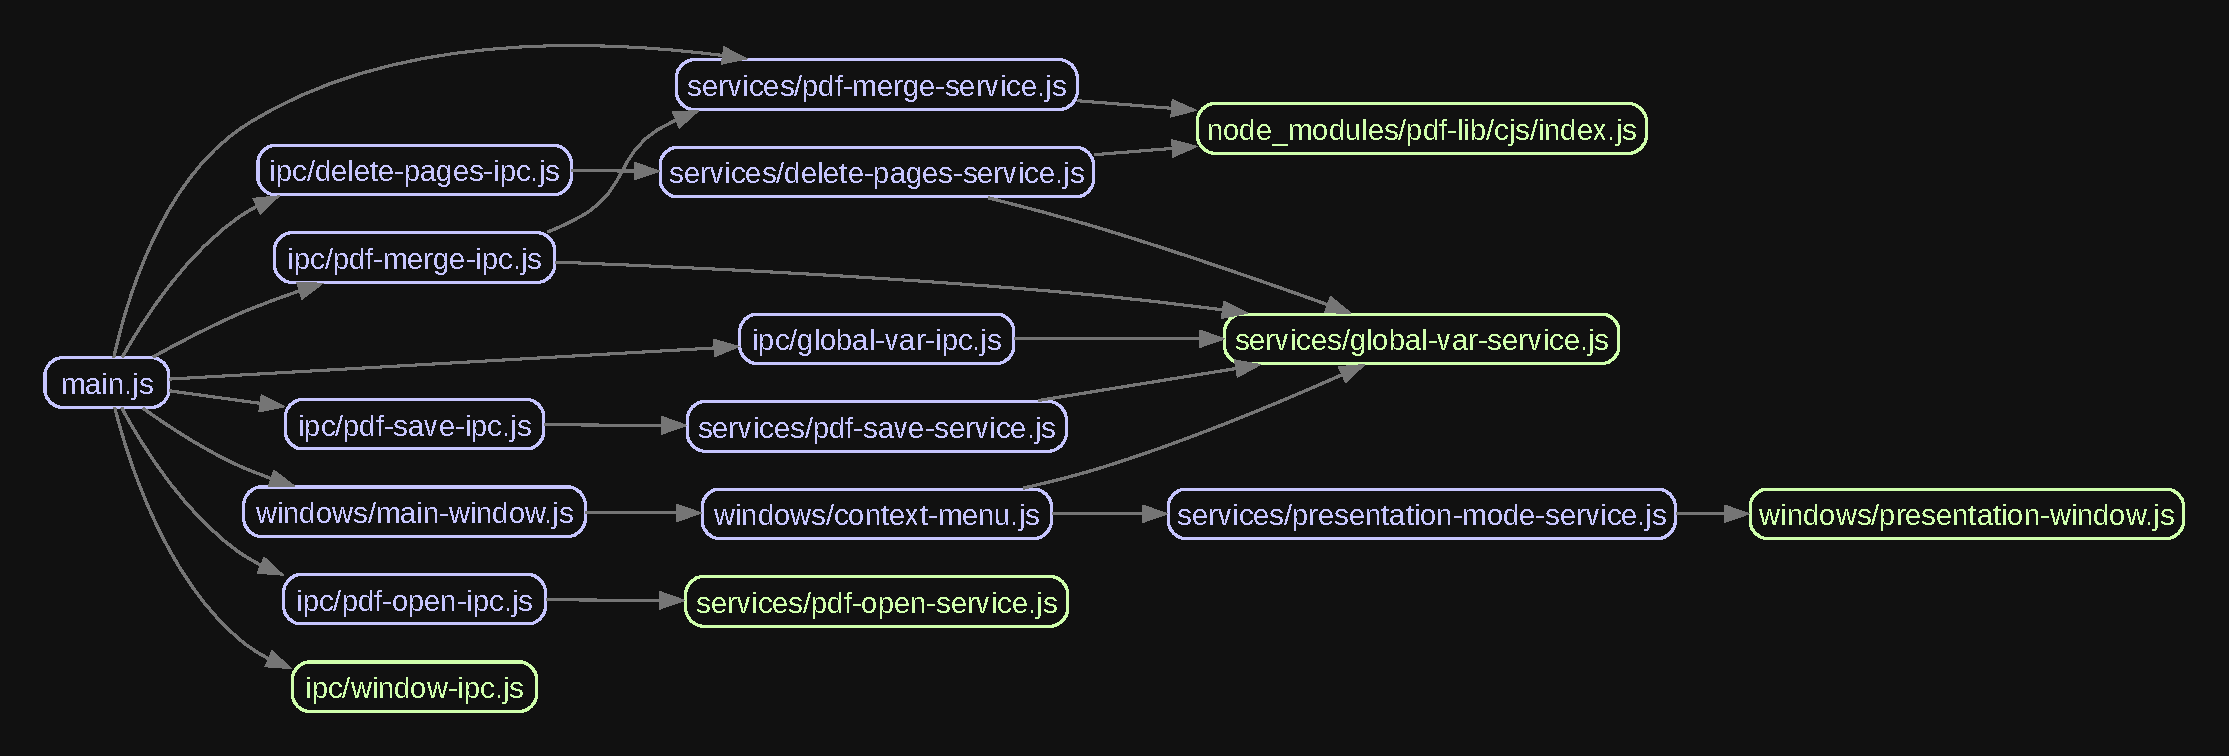
\includegraphics[width=\linewidth]{project/images/dd_main.pdf}}{}
	\caption{\textbf{Diagrama de Dependencias: proceso principal}}
	\label{DiagramaDependenciaMain}
\end{figure}

\subsubsection{Proceso renderer}

\begin{figure}[H]
	\centering
	\IfFileExists{project/images/dd_renderer.pdf}{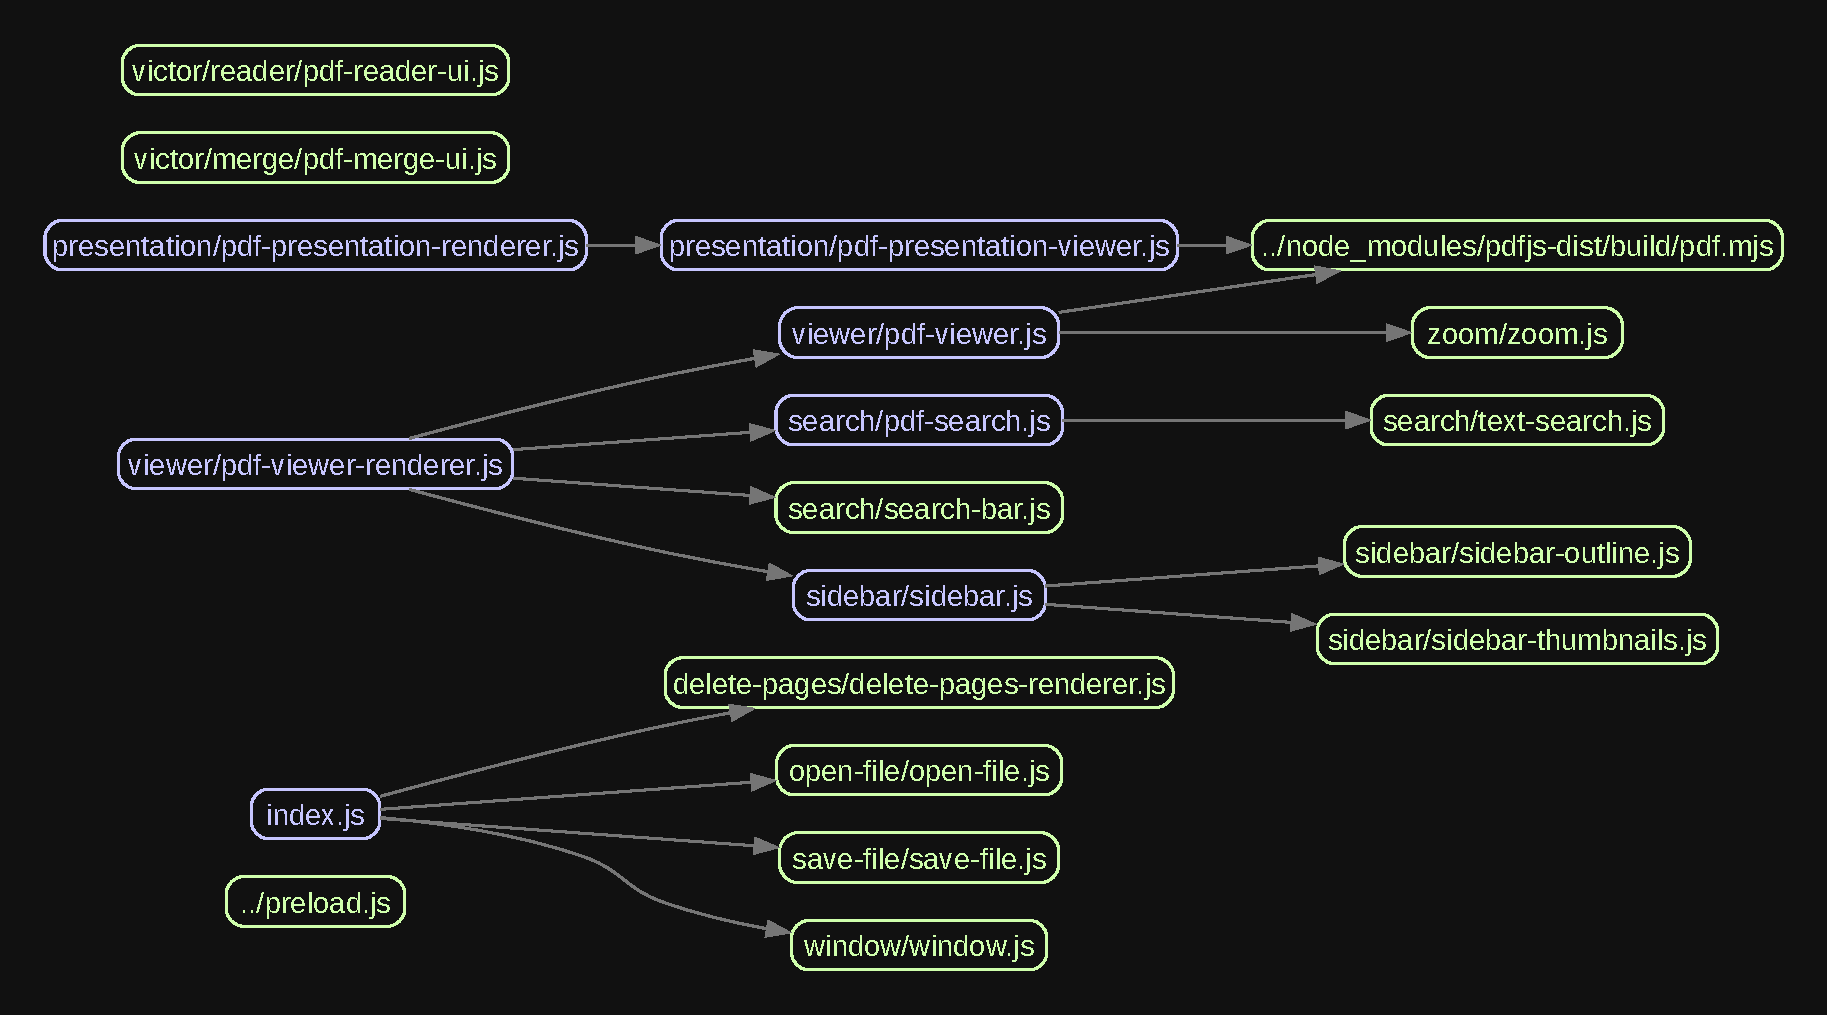
\includegraphics[width=\linewidth]{project/images/dd_renderer.pdf}}{}
	\caption{\textbf{Diagrama de Dependencias: proceso renderer}}
	\label{DiagramaDependenciaRenderer}
\end{figure}


\subsection{Diagrama de bloques}

El diagrama de bloques muestra la organización de los módulos del proyecto y cómo se comunican entre sí de forma superficial. Este diagrama es útil para entender la estructura del proyecto ya que la jerarquía de módulos es similar a la estructura de archivos que tiene el proyecto.

El diagrama (Ver figura \ref{DiagramaBloques}) expone 2 bloques principales: proceso principal y renderer. El bloque del proceso principal tiene el módulo "windows" que tiene ventanas del sistema, el módulo "services" que tiene módulos con funcionalidades del programa y el módulo "ipc" que expone módulos del proceso principal al proceso renderer. El bloque del proceso renderer tiene 2 módulos: index y presentation, cada corresponde a una página de la interfaz de la aplicación.

\begin{figure}[H]
	\centering
	\IfFileExists{project/images/BlockDiagram.pdf}{\includegraphics[width=\linewidth]{project/images/BlockDiagram.pdf}}{}
	\caption{\textbf{Diagrama de Bloques}}
	\label{DiagramaBloques}
\end{figure}

\subsection{Diagrama de Clases}

El diagrama de clases describe las clases que existen dentro de la aplicación. El diagrama (Ver figura \ref{DiagramaClases}) muestra 3 clases. La clase PdfViewer es la encargada de mostrar el pdf dentro de la aplicación, además muestra información como número de página actual y tiene herramientas como el zoom. La clase AnnotationManager se encarga de gestionar y renderizar las anotaciones del documento, esta clase es instanciada por PdfViewer para delegar y modularizar esas responsabilidades. La clase PresentationViewer se encarga de mostrar el pdf en modo presentación.

\begin{figure}[H]
	\centering
	\IfFileExists{project/images/ClassDiagram.pdf}{\includegraphics[width=\linewidth]{project/images/ClassDiagram.pdf}}{}
	\caption{\textbf{Diagrama de Clases}}
	\label{DiagramaClases}
\end{figure}


% project/installation.tex
\chapter{Instrucciones de Instalación}

\section{Entorno de Desarrollo}

\subsection{Dependencias}
La aplicación está construida con el framework Electron que necesita el entorno de ejecución Node.js. Además, la aplicación utiliza bibliotecas de npm para algunas funcionalidades, así que también se debe descargar esa herramienta.

Lista de pasos para preparar el entorno de desarrollo:
\begin{enumerate}
	\item \textbf{Github} El repositorio del proyecto se encuentra en Github. Para trabajar colaborativamente en el repositorio necesita registrarse en este servicio. \url{https://github.com/}.

	\item \textbf{Git} El administrador de versiones del proyecto es Git. Para descargarlo siga las instrucciones en \url{https://git-scm.com/install/}.

	\item \textbf{VSCode} El editor de texto sugerido para desarrollar el proyecto es VSCode. Para descargarlo siga las instrucciones en \url{https://code.visualstudio.com/download}.

	\item \textbf{Node.js y NPM} Descargue la versión más reciente de Node.js siguiendo las instrucciones en \url{https://nodejs.org/es/download}.

\end{enumerate}


\subsection{Código fuente}
Lista de pasos para descargar el código fuente y configurar lo necesario para empezar a trabajar:

\begin{enumerate}
	\item \textbf{Acceder al repositorio} Pida a un administrador del proyecto que le conceda permisos para trabajar en el repositorio del proyecto.

	\item \textbf{Descargar código fuente} Puede descargar el código fuente de varias maneras. El comando `git clone` puede descargar el código del repositorio si git cuenta con los credenciales de Github. Para hacerlo puede seguir la guía en \url{https://docs.github.com/en/get-started/git-basics/caching-your-github-credentials-in-git}

	\item \textbf{Descargar Electron y otras bibliotecas} Ejecute el comando `npm ci` en la carpeta raíz del proyecto.

	\item \textbf{Descargar formatter}: Descargue Prettier en su editor de texto para que el código siga el formato definido. VSCode cuenta una externsión que configura Prettier de forma automática. También, se recomienda instalar ESLint para detectar errores en el código, VSCode también tiene una extensión para está herramienta.

	\item \textbf{Estándar de código}: Antes de programar lea el documento en "docs/standard.md". Este documento tiene una lista de buenas prácticas que se deben seguir en el desarrollo de la aplicación.

	\item \textbf{Ejecutar aplicación en entorno de desarrollo}: Para ejecutar la aplicación usando el código fuente utilice el comando `npm start`.

\end{enumerate}

\section{Entorno de Producción}

\subsection{Instrucciones de compilación}
Para compilar el proyecto se ejecuta el comando `npm run build`. Este comando usa la biblioteca electron-builder para compilar y empaquetar el proyecto en un ejecutable portable para las plataformas: Windows y Linux. Esta biblioteca también genera un instalador del programa para la plataforma Windows. Es importante resaltar que la compilación cruzada no funciona debido a las bibliotecas criptográficas que se utilizan para la firma digital.

\subsection{Dependencias}
El proceso de compilación empaqueta todas las dependencias necesarias en el ejecutable, por lo tanto el entorno de producción solo necesita tener el binario.

\subsubsection{Dependencia para abrir archivos DVI}
La apertura de archivos DVI (US-041) requiere el conversor \texttt{dvipdfmx}, disponible en TeX Live o MiKTeX. Después de instalarlo, verifique que esté disponible en \texttt{PATH}. También puede indicar la ruta del ejecutable mediante la variable de entorno \texttt{DVIPDFMX\_PATH} antes de iniciar Folio.

\subsection{Instrucciones de instalación}
El ejecutable es portable, así que no requiere instalarse en el sistema. Para ejecutar la aplicación solo debe correr el ejecutable.

El instalador para Windows instala el programa en el sistema. Al ejecutarlo, se despliegan opciones sobre la ruta de instalación, entre otras, estas opciones dependen de las preferencias del usuario.


% project/api.tex
%\chapter{Métodos del API}
%En esta sección detalle los métodos que tiene publicados en la sección back-end de su sistema.
%Por cada método incluya parámetros necesarios, formato de envío, y cualquier otro procedimiento necesario para comprender y utilizar correctamente su API.
%
%Puede utilizar este como ejemplo:
%\url{https://library.vuforia.com/articles/Solution/How-To-Use-the-Vuforia-Web-Services-API.html}
%
%


% project/conclusion.tex
\chapter{Conclusiones y trabajo futuro}
\section{Conclusiones}

%Documente el aprendizaje acumulado durante el desarrollo del proyecto. Las conclusiones deben ser hechos concretos que puedan ser de utilidad para un lector externo que no conoce el proyecto.

El proceso renderer no cuenta con una forma de persistir datos pesados en memoria entre páginas o entre refrescos. Ya que el proceso renderer ejecuta Chromium las formas de guardar datos son el localStorage o sessionStorage, pero no son eficientes y tienen límites pequeños (<10MB). Por lo tanto, la solución a este problema es mantener la información persistente en el proceso principal y hacer que el proceso renderer la extraiga cuando lo necesita. Este método tiene la ventaja de que también permite compartir información entre varios procesos renderer (varias ventanas de la aplicación). Es importante resaltar que la comunicación entre procesos conlleva un overhead, sin embargo en este proyecto se procesan pocos datos(<1GB) y la latencia(<500ms) no es un aspecto importante.


La implementación de "lazy loading" en el visor de archivos PDFs resultó crucial. Previo a su implementación, con un archivo PDF pesado la aplicación utilizaba alrededor de 2.9GB de memoria una vez cargado el PDF completo. Tras la implementación de lazy loading el mismo archivo consumía alrededor de 700MB de memoria. El problema que surge de esto es que las páginas se deben volver a renderizar cada vez que entran en pantalla lo que puede causar que se muestren páginas en blanco hasta que carguen, aunque esto solo debería ocurrir si las páginas son muy pesadas o después de un salto con la funcionalidad de salto de página o búsqueda de palabras.


A la hora de empezar un sprint es importante verificar que las historias de usuario tengan la menor dependencia entre sí. Durante el desarrollo de este proyecto, la historia de navegar el outline y la de reordenar páginas dependían completamente del sidebar, un panel lateral que contiene tanto las miniaturas de las páginas como el outline del documento. Por ende, 2 compañeros estuvieron "pegados" hasta que el desarrollador encargado del outline pudo terminar su historia de usuario. Cuando varias historias dependen de un mismo componente, conviene sacarlo a una historia aparte y hacerla de primera en el sprint.


\section{Problemáticas y limitaciones}
%Recuerde que sólo debe registrar aquellas problemáticas que el sistema TIENE, no debe mencionar problemas que aparecieron durante el desarrollo, pero que se resolvieron adecuadamente.
%Considere como problemáticas errores o comportamientos indeseables que el sistema tiene. Por ejemplo fugas de memoria, puntos en los que el sistema se cuelga, etc...
%Limitaciones por el otro lado, son cosas que el sistema NO puede hacer, ya sea por diseño o por que se quería incluir pero no fue posible. Por ejemplo la falta de multijugador por Internet es una limitación, también liste aquí las plataformas para las cuales el sistema está diseñado (sistema operativo, requerimientos mínimos, resolución recomendada, etc...).

\subsubsection{Problemáticas}

El tiempo de arranque de la aplicación es una problemática presente. Usualmente tarda más de 2 segundos en aparecer la ventana en pantalla, esto sin estar cargando ningún pdf.

La búsqueda de texto presenta errores en documentos con formato IEEE de doble columna. Al buscar un término en estos documentos, las coincidencias pueden no encontrarse o resaltarse de forma incorrecta.

Actualmente las acciones rápida con teclas tienen conflictos con la funcionalidad de búsqueda de palabras pues estas siguen activas mientras se trata de usar esta función, haciendo que el programa se controle de manera extraña.

\subsubsection{Limitaciones}



Los requerimientos mínimos del sistema son los siguientes:
\begin{itemize}
	\item \textbf{RAM: }200MB. Esta es la memoria para el programa base, si se carga un pdf entonces se necesita al menos una cantidad de memoria igual al tamaño del archivo.
	\item \textbf{Almacenamiento:} 250 MB. Tamaño del ejecutable de la aplicación.
	\item \textbf{Procesamiento:} Un procesador Intel i8 serie 8000 o similar. Es probable que funcione con menos procesamiento pero no ha sido probado.
	\item \textbf{Sistema operativo:} Se compilan ejecutables para los sistemas operativos Windows 11 y cualquier distribución de Linux que soporte el formato AppImage.
\end{itemize}


\section{Trabajo futuro}

Se recomienda implementar un documento de estilo global para normalizar aspectos del estilo a lo largo de la aplicación. Esto mejora la estética de la aplicación y facilita el desarrollo.

Se puede implementar una interfaz web del sistema.

Se puede implementar gestión de múltiples firmas con bloqueo de concurrencia. (Investigar acerca de Docusign).


%%%Texto explicativo, no debe aparecer en el documento final
%\section{NOTAS SOBRE LAS REFERENCIAS BIBLIOGRÁFICAS}
%En el archivo references.bib puede agregar las fuentes bibliográficas usadas en el documento en formato \emph{bibtex}.
%Puede incluir fuentes que no citó en el archivo de referencias. Aquellas que no citó automáticamente serán omitidas en la lista de referencias.
%Para citar una referencia en el texto debe usar el comando \emph{cite}.
%
%Por ejemplo el artículo de Dean se cita usando \cite{dean2003}.
%Note cómo los libros de Ortíz y Sánchez no salen en las referencias.
%
%\emph{Procure eliminar esta sección de su documento}
%%%Aquí termina el texto explicativo


% project/ref.tex


\bibliographystyle{apacite}
\bibliography{folio-manual-references}


\end{document}